\chapter{Ispitivanje razvijenog sklopovskog rješenja}
U postupku provjere realiziranog rješenja ispitani su sustavi za napajanje, žična komunikacija između dijelova sustava, bežična komunikacija, upisivanje korisničkog programa u Flash memoriju mikrokontrolera, snimanje zvuka, pohrana podataka na SD karticu, RTC, komunikacija s PPG senzorom i mjerenje impedancije kože.

U svim testovima korišten je multimetar za mjerenje napona i osciloskop za promatranje signala u komunikacijama između sustava. Za ispitivanje napajanja korišteni su USB strujni adapter koji podržava mogućnost brzog punjenja, različite litij-ionske baterije u 18650 kućištu i USB ispitivač UT658DUAL tvrtke Changan UNI-T, prikazan na slici \ref{slk:UT658DUAL}. Ovaj uređaj se može spojiti između USB izvora i uređaja te pokazuje razinu napona, jakost struje koju izvor daje, količinu potrošenog naboja u mAh i vrijeme trajanja mjerenja.
\begin{figure}[htb]
    \centering
    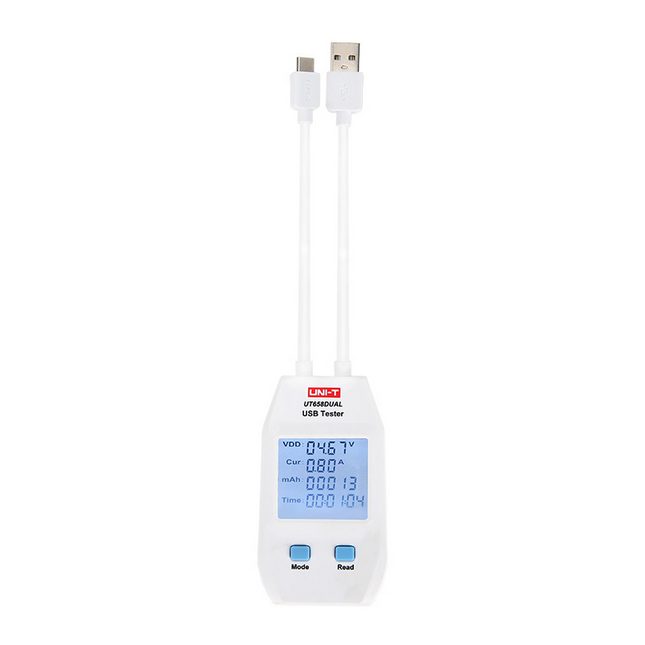
\includegraphics[width=6 cm]{Figures/UT658DUAL.png}
    \caption{USB ispitivač UT658DUAL}
    \label{slk:UT658DUAL}
\end{figure}
\section{Središnji uređaj}
Na slikama \ref{slk:MB_TEST_01} i \ref{slk:MB_TEST_02} prikazano je ispitivanje središnjeg uređaja. Umjesto priključka za bateriju, priključen je držač za standardnu 18650 bateriju radi lakšeg testiranja. Naime, baterija se često vadi i stavlja tijekom testiranja, a odabrani priključak predviđen je da se rijetko odspaja pa ga je stoga i teško odspajati veći broj puta tijekom ispitivanja.
\begin{figure}[htb]
    \centering
    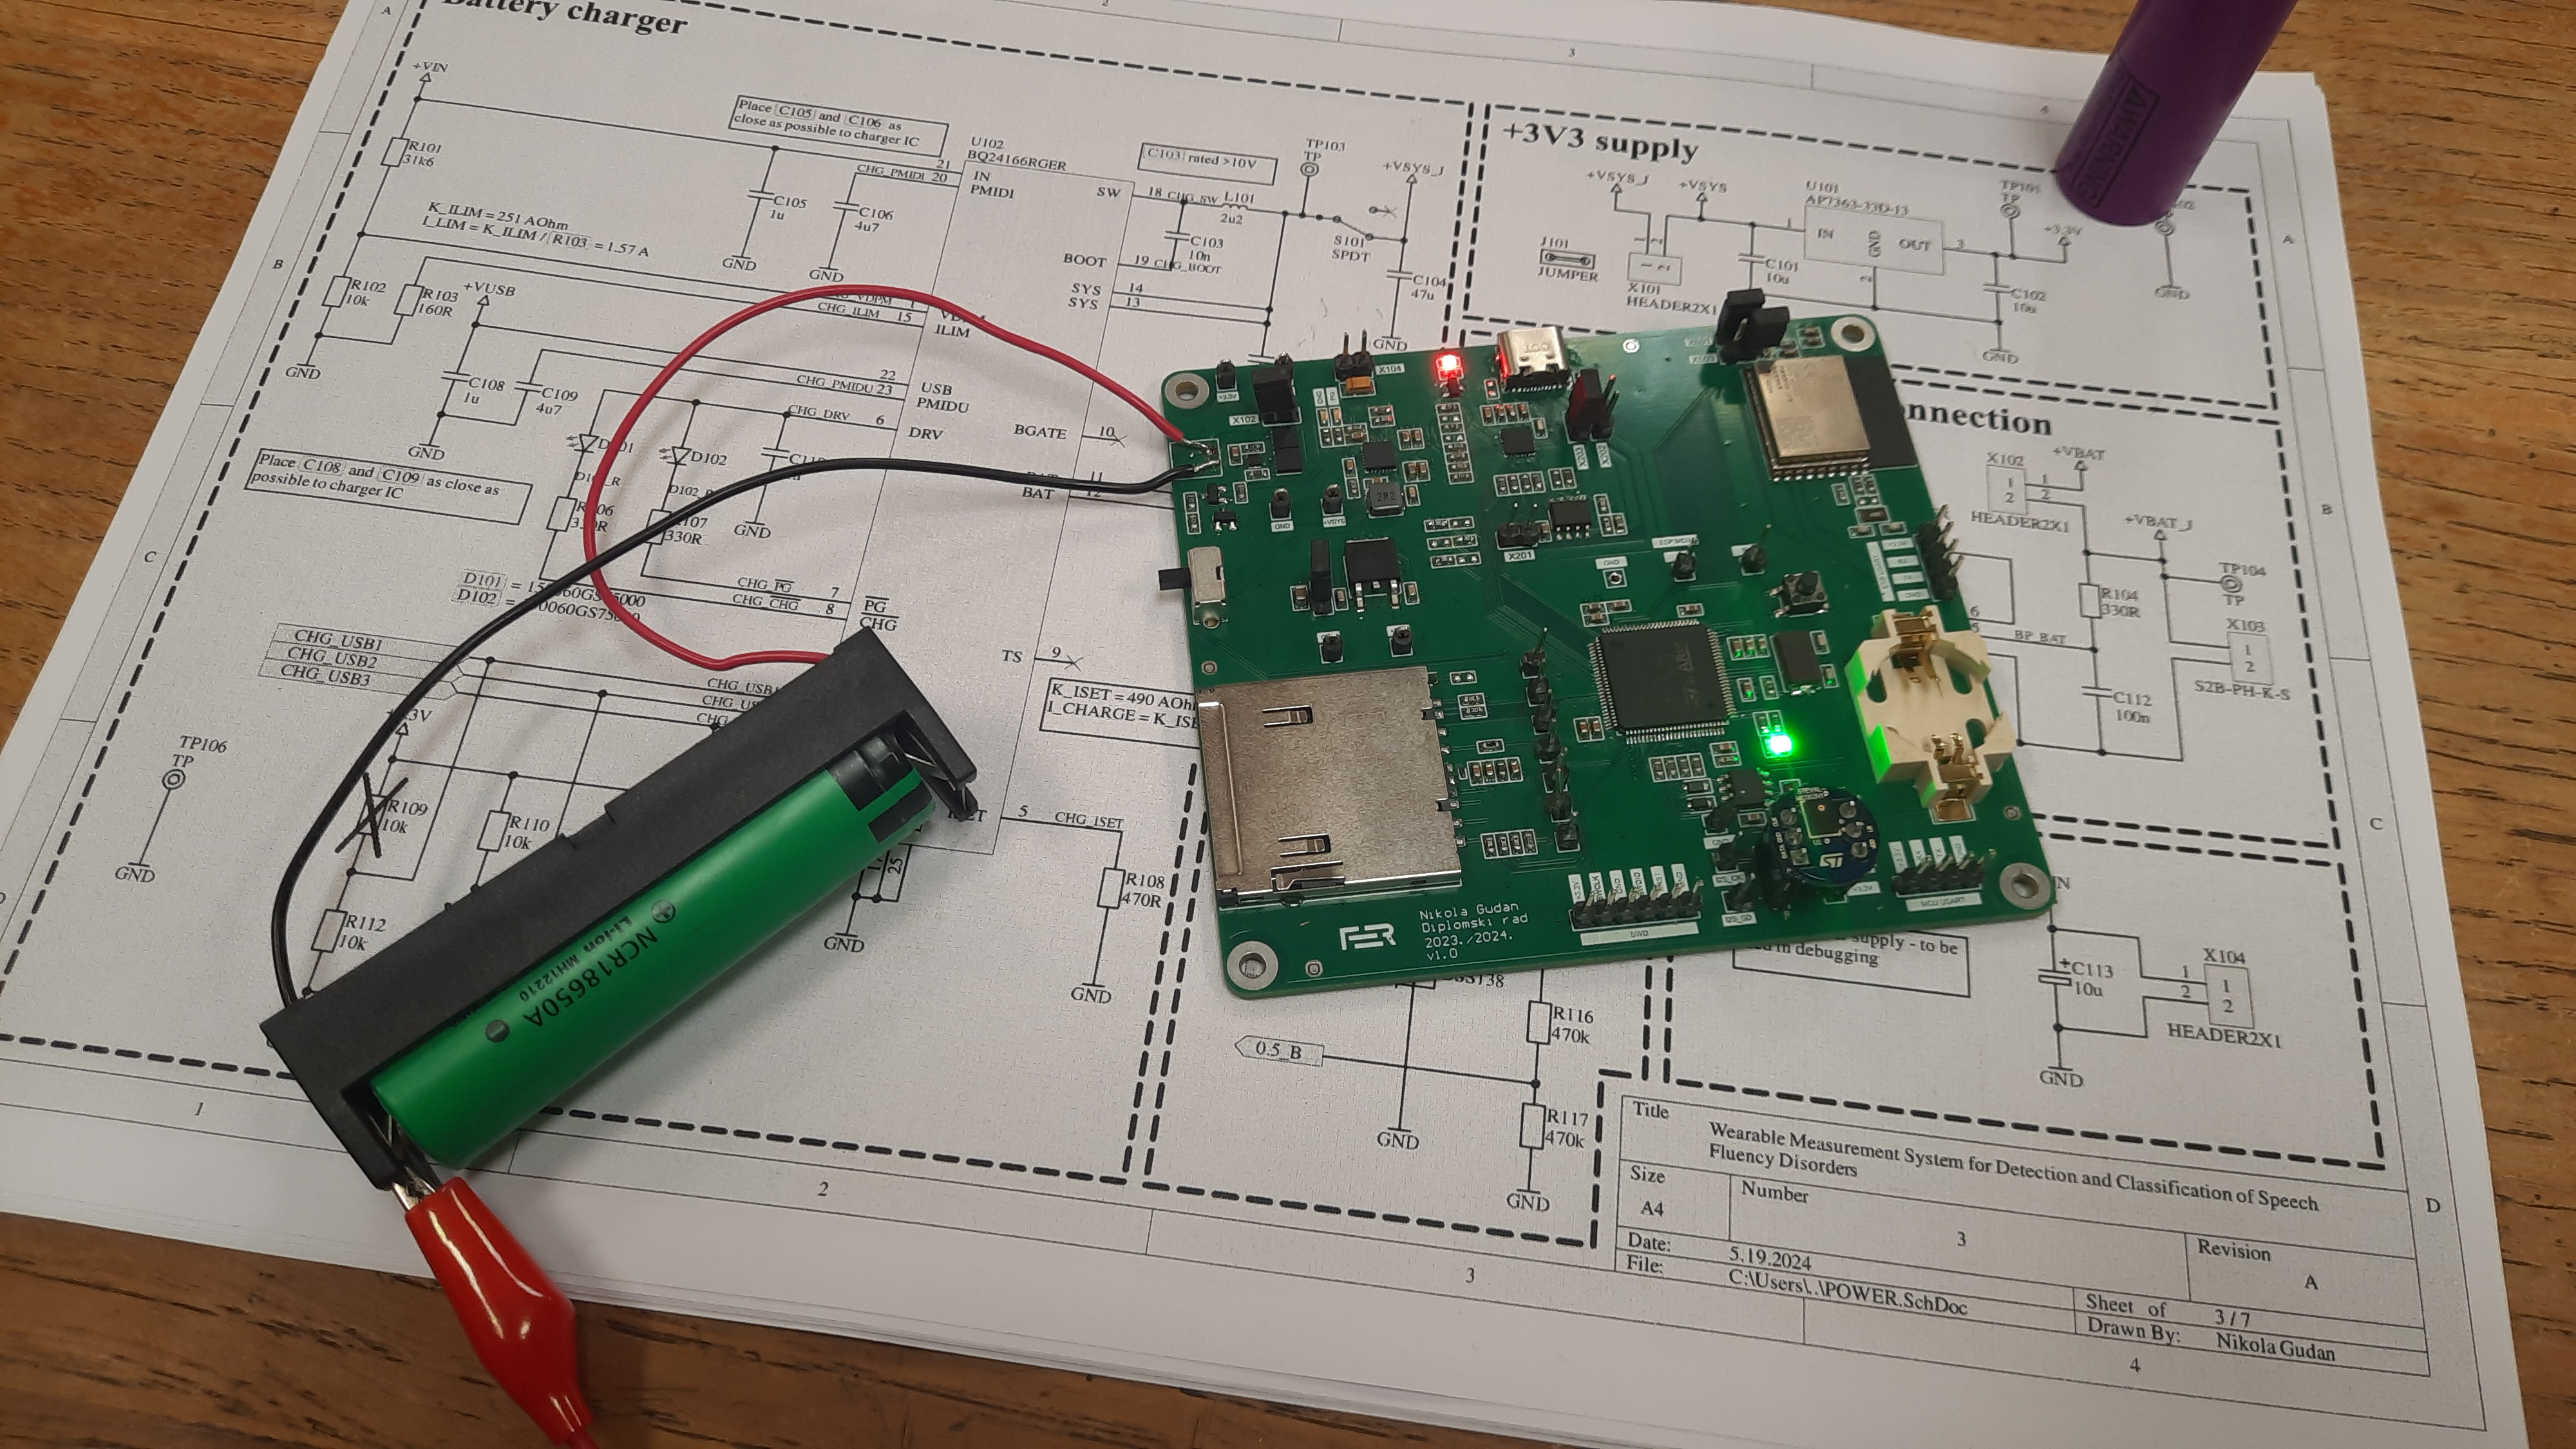
\includegraphics[width=10 cm]{Figures/MB_TEST_01.jpg}
    \caption{Ispitivanje pločice središnjeg uređaja}
    \label{slk:MB_TEST_01}
\end{figure}
\begin{figure}[htb]
    \centering
    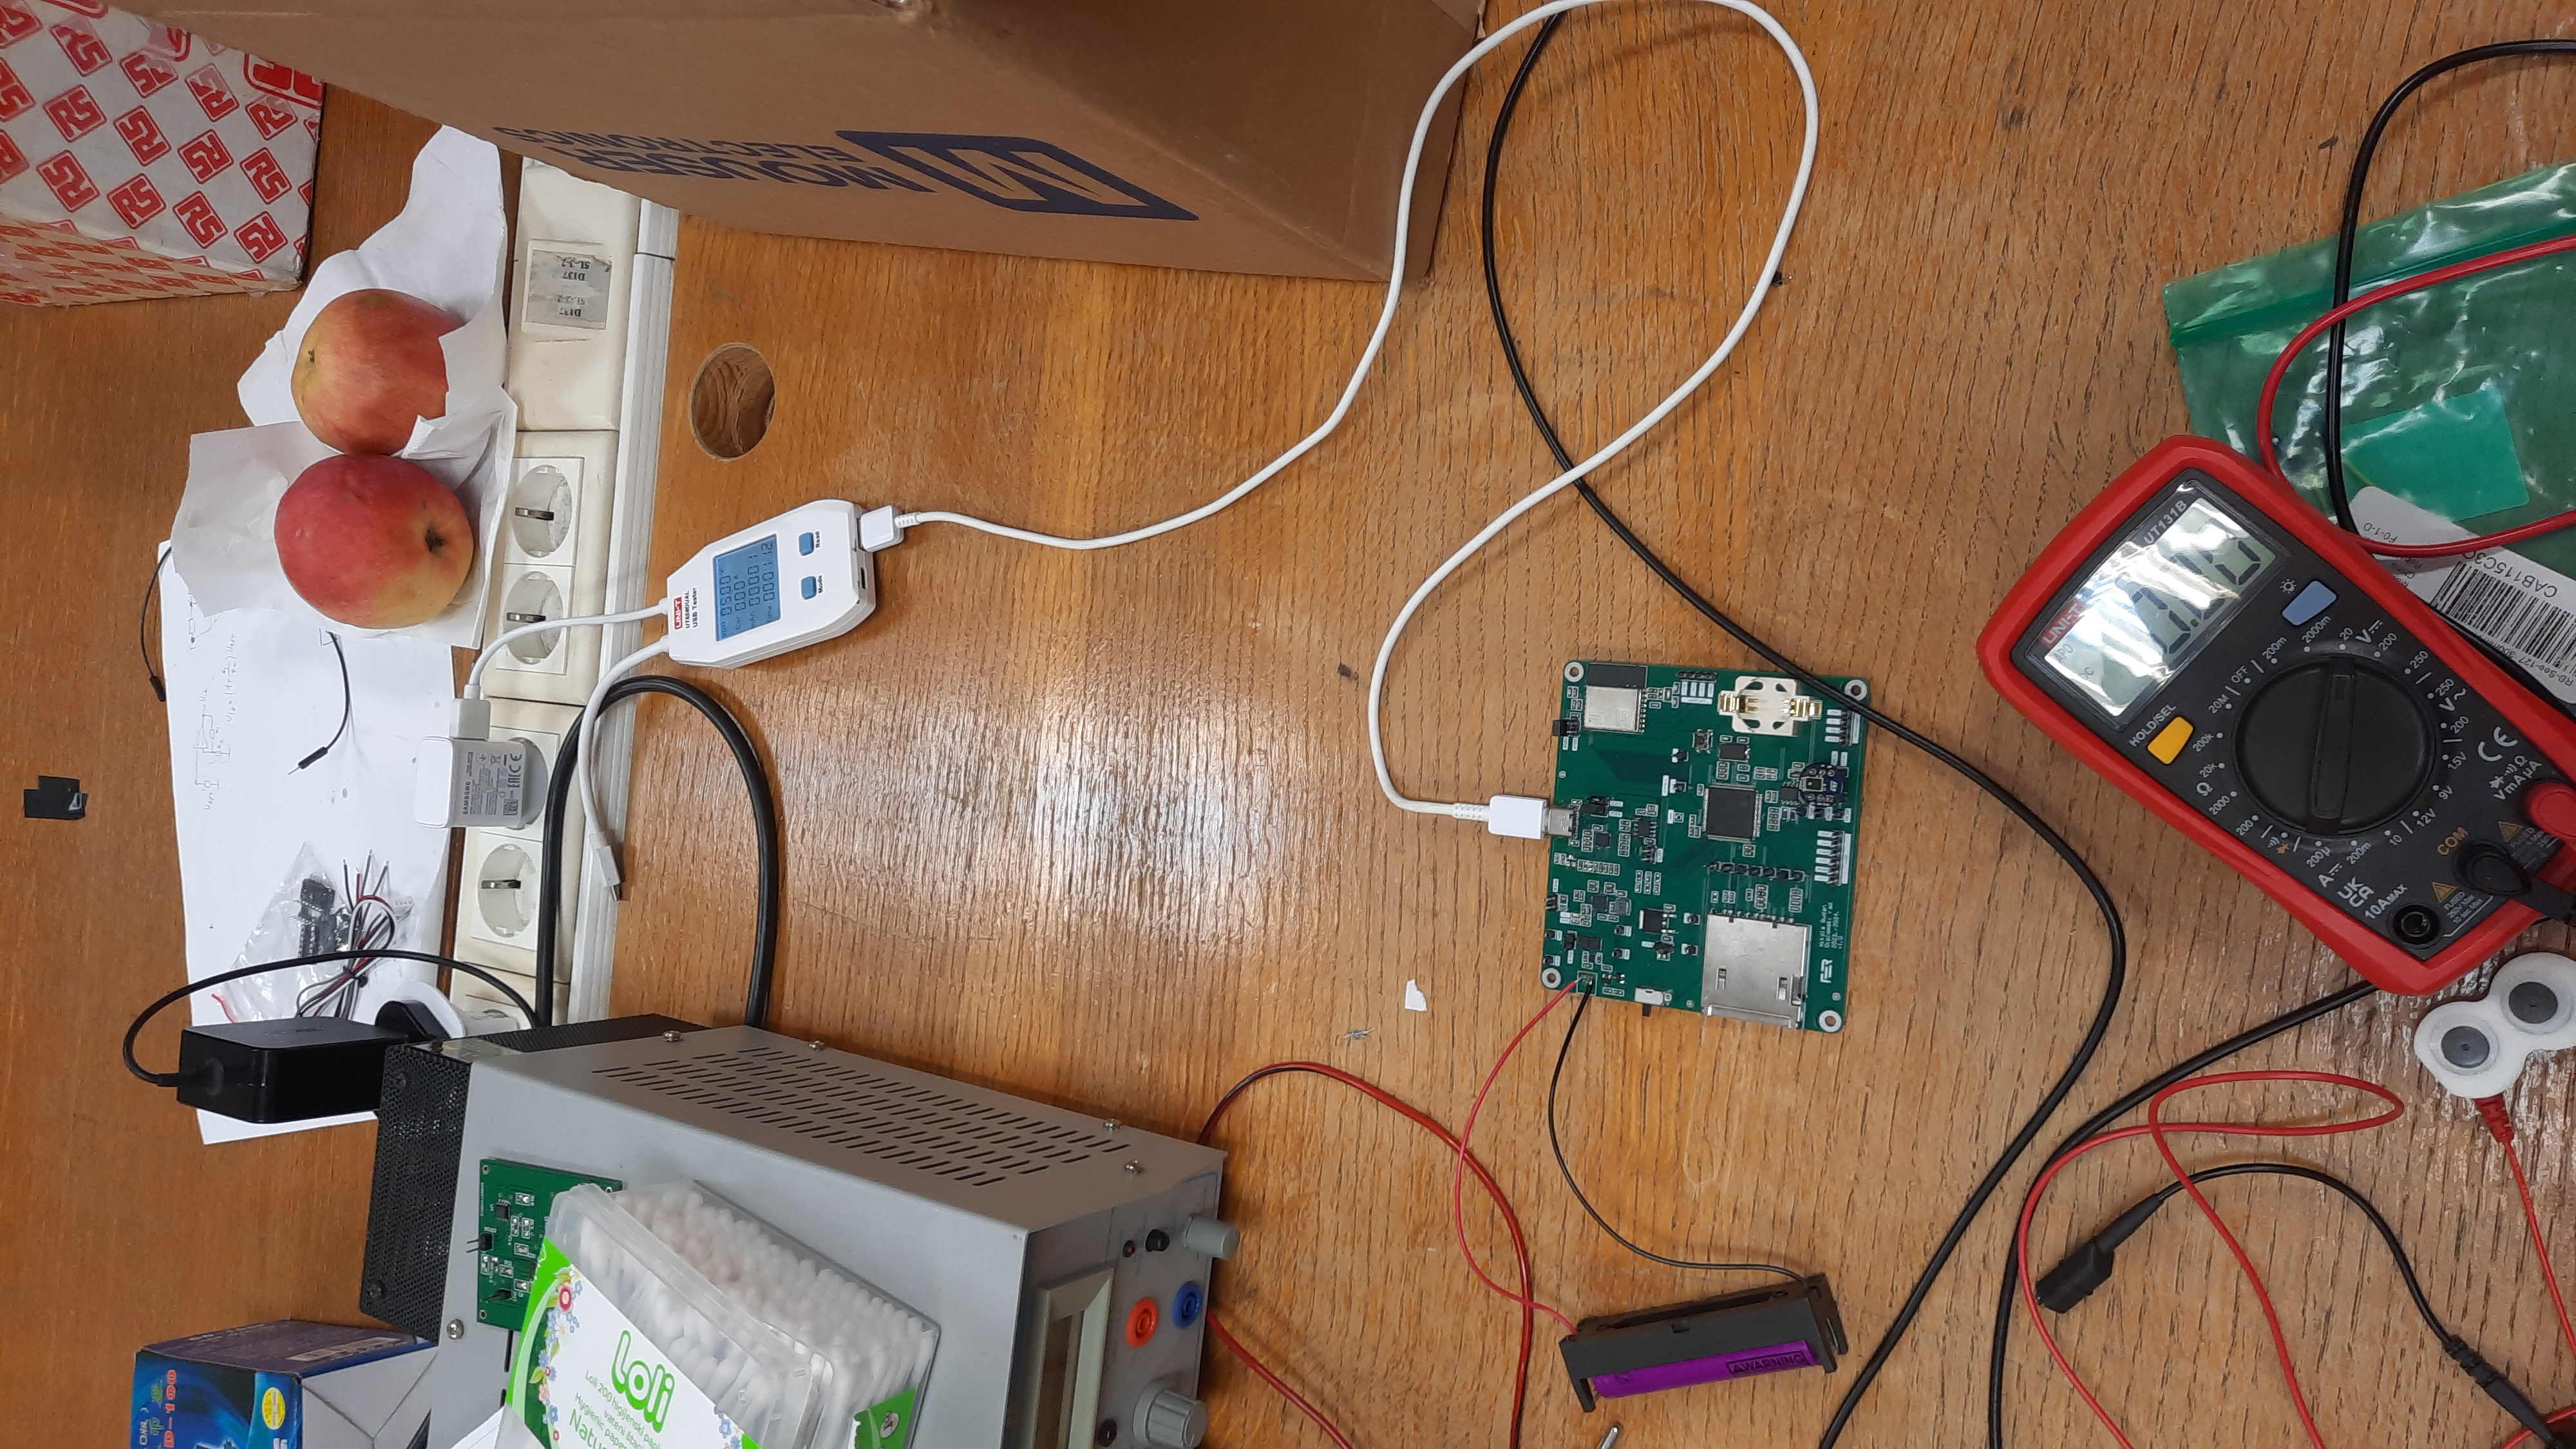
\includegraphics[width=10 cm]{Figures/MB_TEST_02.jpg}
    \caption{Postav ispitivanja pločice središnjeg uređaja}
    \label{slk:MB_TEST_02}
\end{figure}

U postupku ispitivanja otkrivena je pogreška u dizajnu USB napajanja. Naime, kada se spoji USB izvor napajanja, bez obzira podržava li izvor zatraženu snagu ili ne, napajanje s USB-a se ne prosljeđuje prema ostatku sustava. Ustanovljeno je da je problem u tranzistorskoj sklopci (slika \ref{slk:MB_USB}). Naime, kada integrirani sklop pokuša uključiti tranzistore, na prvom tranzistoru dolazi do pada napona na diodi koja se nalazi unutar tranzistora pa se na uvodu drugog tranzistora nalazi napon napajanja umanjen za napon provoda diode (između 0.5 V i 1.2 V \cite{di:dmp3098}). Integrirani sklop je preko VDC\_OUT stezaljke detektirao previsok pad napona i onemogućio napajanje s USB-a. Radi toga su napravljene izmjene u USB napajanju kod narukvice, koje su vidljive na slici \ref{slk:BR_USB}.

Kada baterija nije bila spojena, nije bilo moguće uključiti USB napajanje iz razloga objašnjenog u potpoglavlju \ref{sec:BR_USB}. Ukratko, integrirani sklop nije mogao postaviti odgovarajuće otpornike na CC linije pa se nije mogla zatražiti nikakva snaga od USB izvora.

Tijekom testiranja punjača utvrđeno je da punjač može bez problema proslijediti napon baterije na izlaz. Međutim, kada se priključio vanjski napon, bilo na USB ili preko priključka za laboratorijski izvor napona u svrhu punjenja baterije, punjač više nije radio. Bilo je vidljivo treperenje svjetlećih dioda za indikaciju ispravnog napajanja i punjenja frekvencijom 1 Hz. Naime, dolazi do aktiviranja temperaturne zaštite na način opisan u potpoglavlju \ref{sec:BR_BATCHG}.

Paralelno s postupkom izrade tiskane pločice, razvijena je programska podrška za središnji uređaj. S obzirom da veći dio podsustava za napajanje, izuzev baterije, nije radio, tijekom testiranja programske podrške, a samim time i digitalnog dijela sustava, uređaj se napajao putem programatora, koji je bio priključen na pločicu cijelo vrijeme tijekom testiranja programske podrške. Utvrđeno je da mikrofon normalno snima govor, da mikrokontroler komunicira sa svim podsustavima i također da bez poteškoća obrađuje i sprema podatke na SD karticu. Utvrđeno je nadalje da se bežični podsustav uspješno može programirati te da RTC mjeri vrijeme uz napajanje s litijske baterije, čime je potvrđeno da digitalni dio sustava u potpunosti radi kako je zamišljeno.

\section{Narukvica}

\begin{figure}[htb]
    \centering
    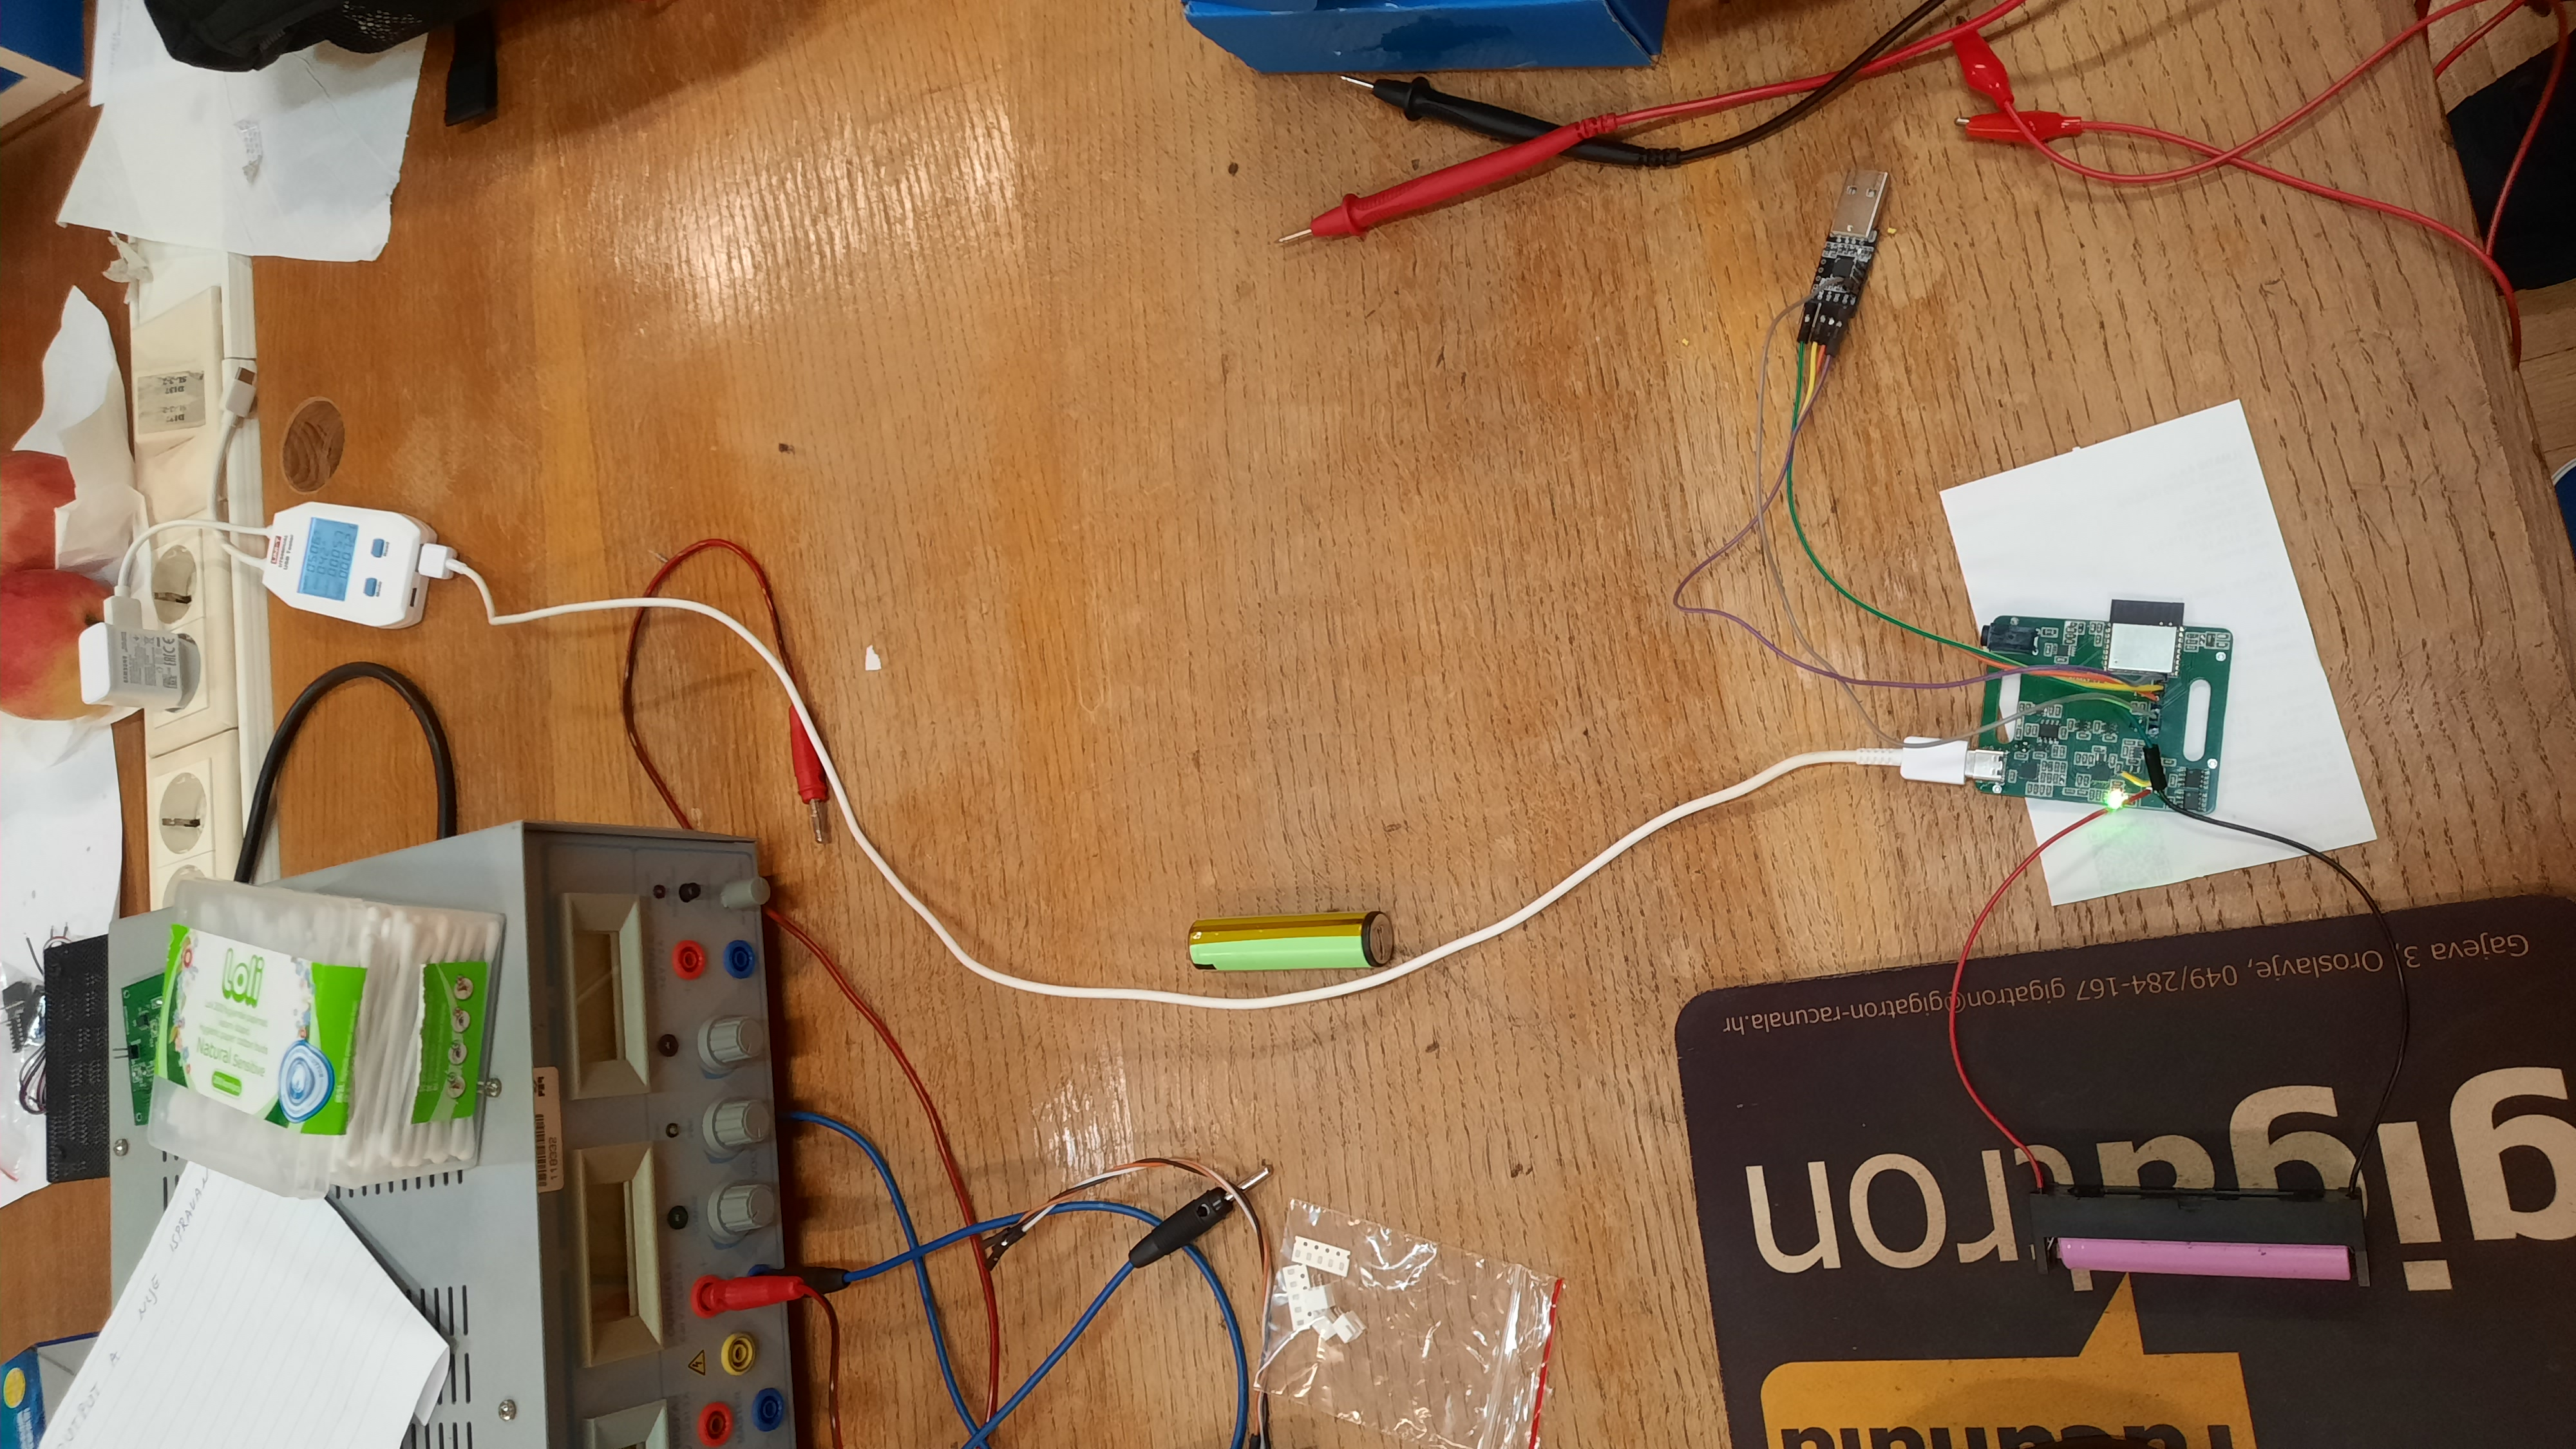
\includegraphics[width=10 cm]{Figures/BR_TEST_02.jpg}
    \caption{Postav ispitivanja pločice narukvice}
    \label{slk:BR_TEST_01}
\end{figure}
\begin{figure}[htb]
    \centering
    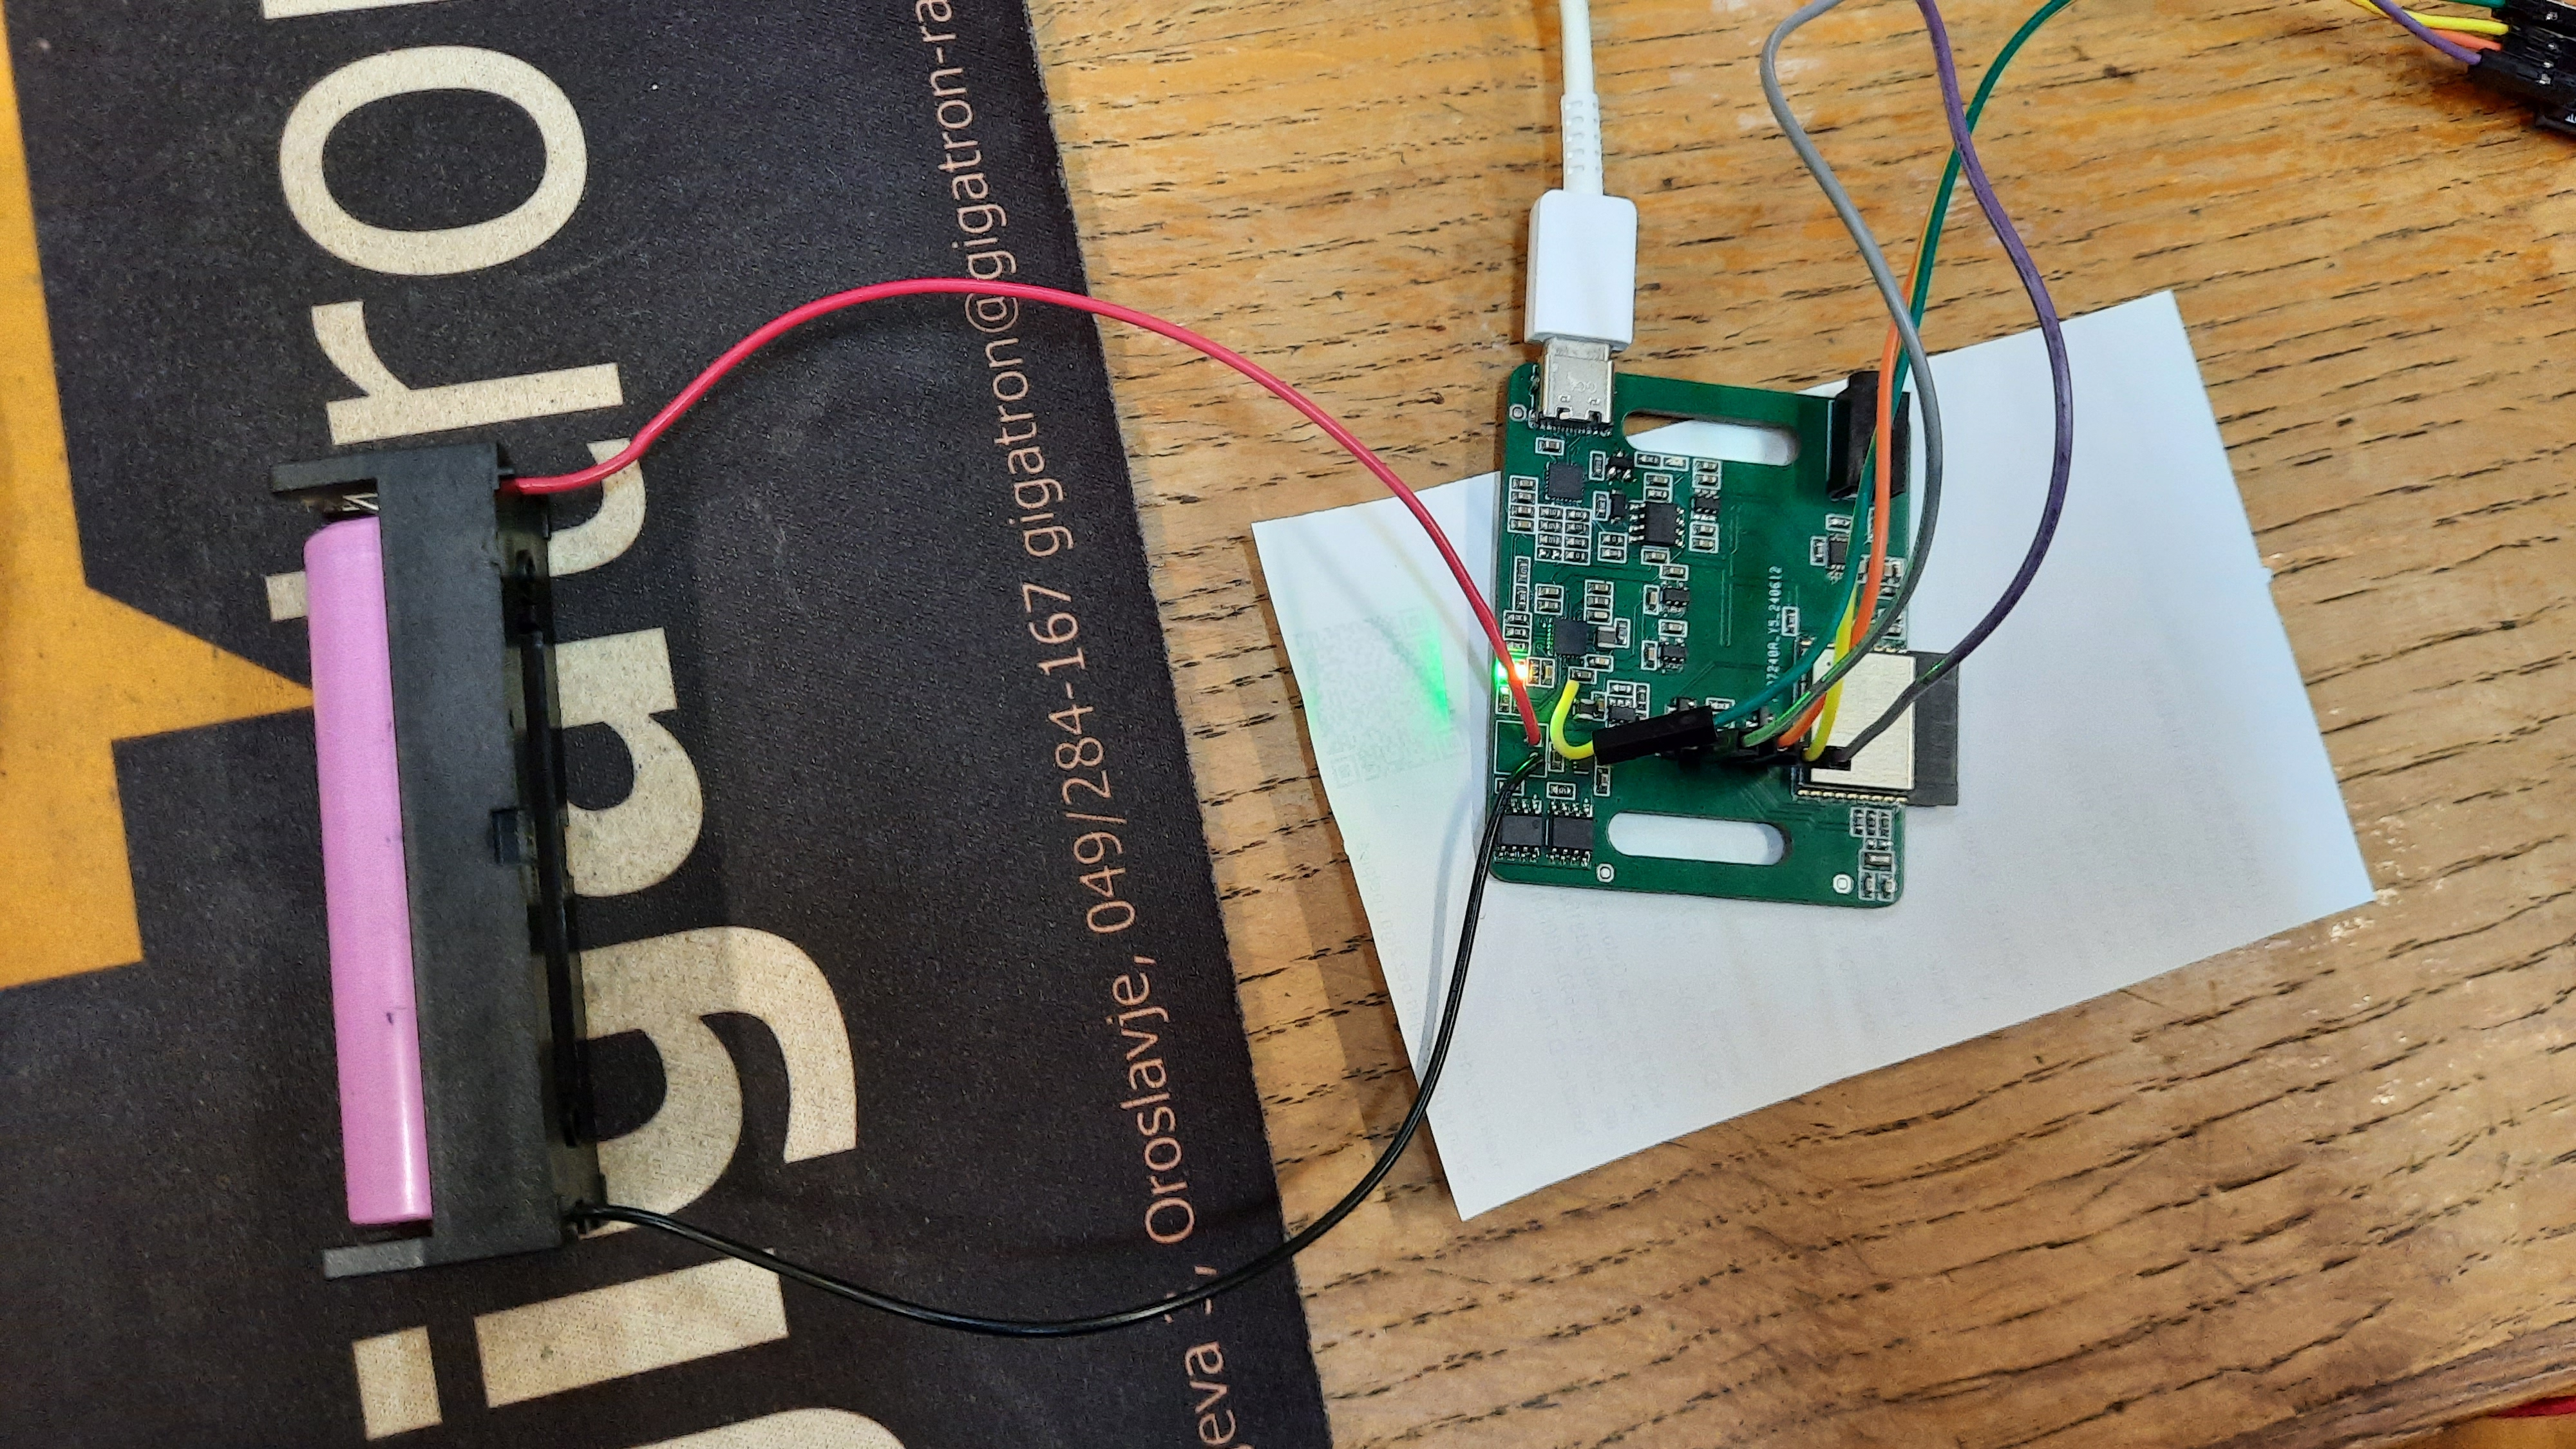
\includegraphics[width=10 cm]{Figures/BR_TEST_01.jpg}
    \caption{Ispitivanje pločice narukvice}
    \label{slk:BR_TEST_02}
\end{figure}

Na temelju ispitivanja središnjeg uređaja, napravljene su izmjene u dizajnu napajanja koje su implementirane na pločici narukvice, kako je opisano u poglavlju \ref{pog:bracelet}. Ispitivanje pločice narukvice prikazano je na slikama \ref{slk:BR_TEST_01} i \ref{slk:BR_TEST_02}.

Tijekom ispitivanja primijećena je pogreška u dizajnu baterijskog napajanja. Ime mreže koja je spojena na pozitivan terminal baterije (slika \ref{slk:BR_BATPROT}) i ime mreže koja je spojena na ulaz za bateriju na punjaču (slika \ref{slk:BR_BATCHG}) su različiti. Radi toga baterija, nakon zaštite, nije pogreškom bila nigdje spojena pa je bilo potrebno te dvije mreže kratko spojiti žicom naknadno, čime je napajanje proradilo.

Podsustav za USB napajanje sada može upravljati napajanjem i kada je na uređaj spojeno samo USB napajanje. Također, narukvica se sada može napajati putem USB-a i kada baterija nije spojena. Baterijski punjač može proslijediti napajanje baterije ili može regulirati napajanje USB-a.
\begin{figure}[htb]
    \centering
    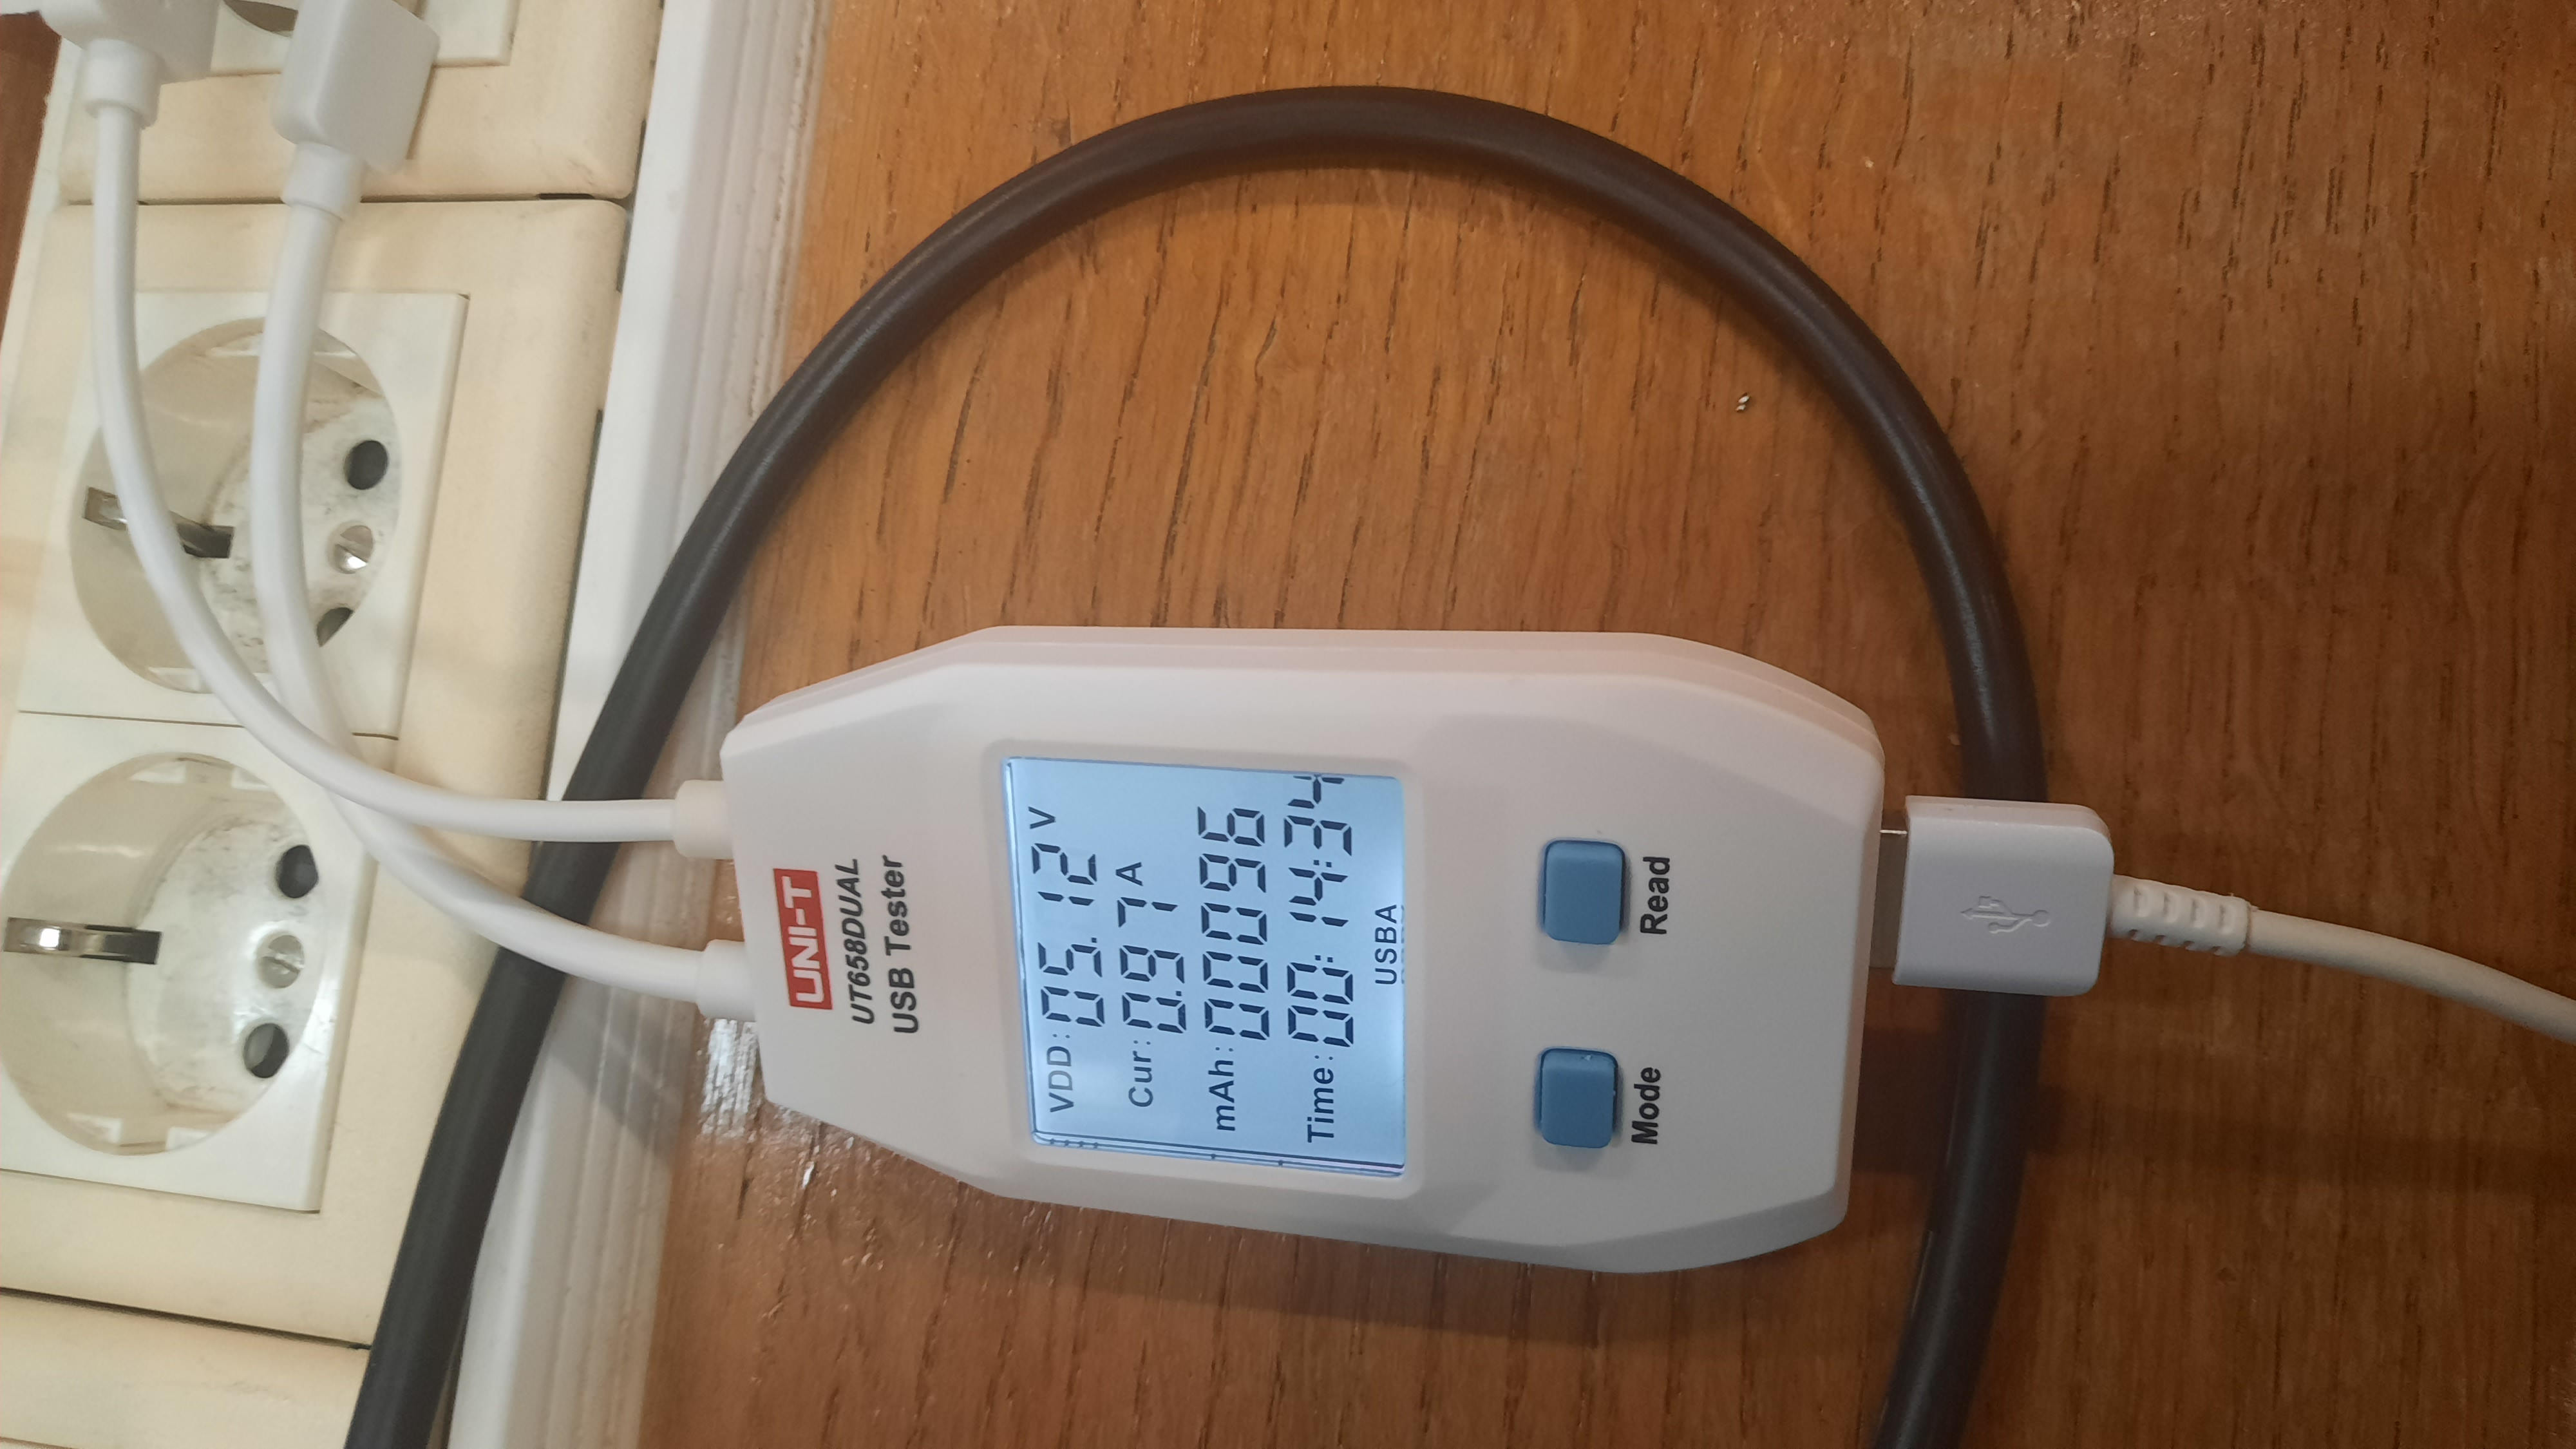
\includegraphics[width=10 cm]{Figures/BR_TEST_04.jpg}
    \caption{Brzo punjenje, punjenje konstantnom strujom}
    \label{slk:BR_TEST_04}
\end{figure}
\begin{figure}[htb]
    \centering
    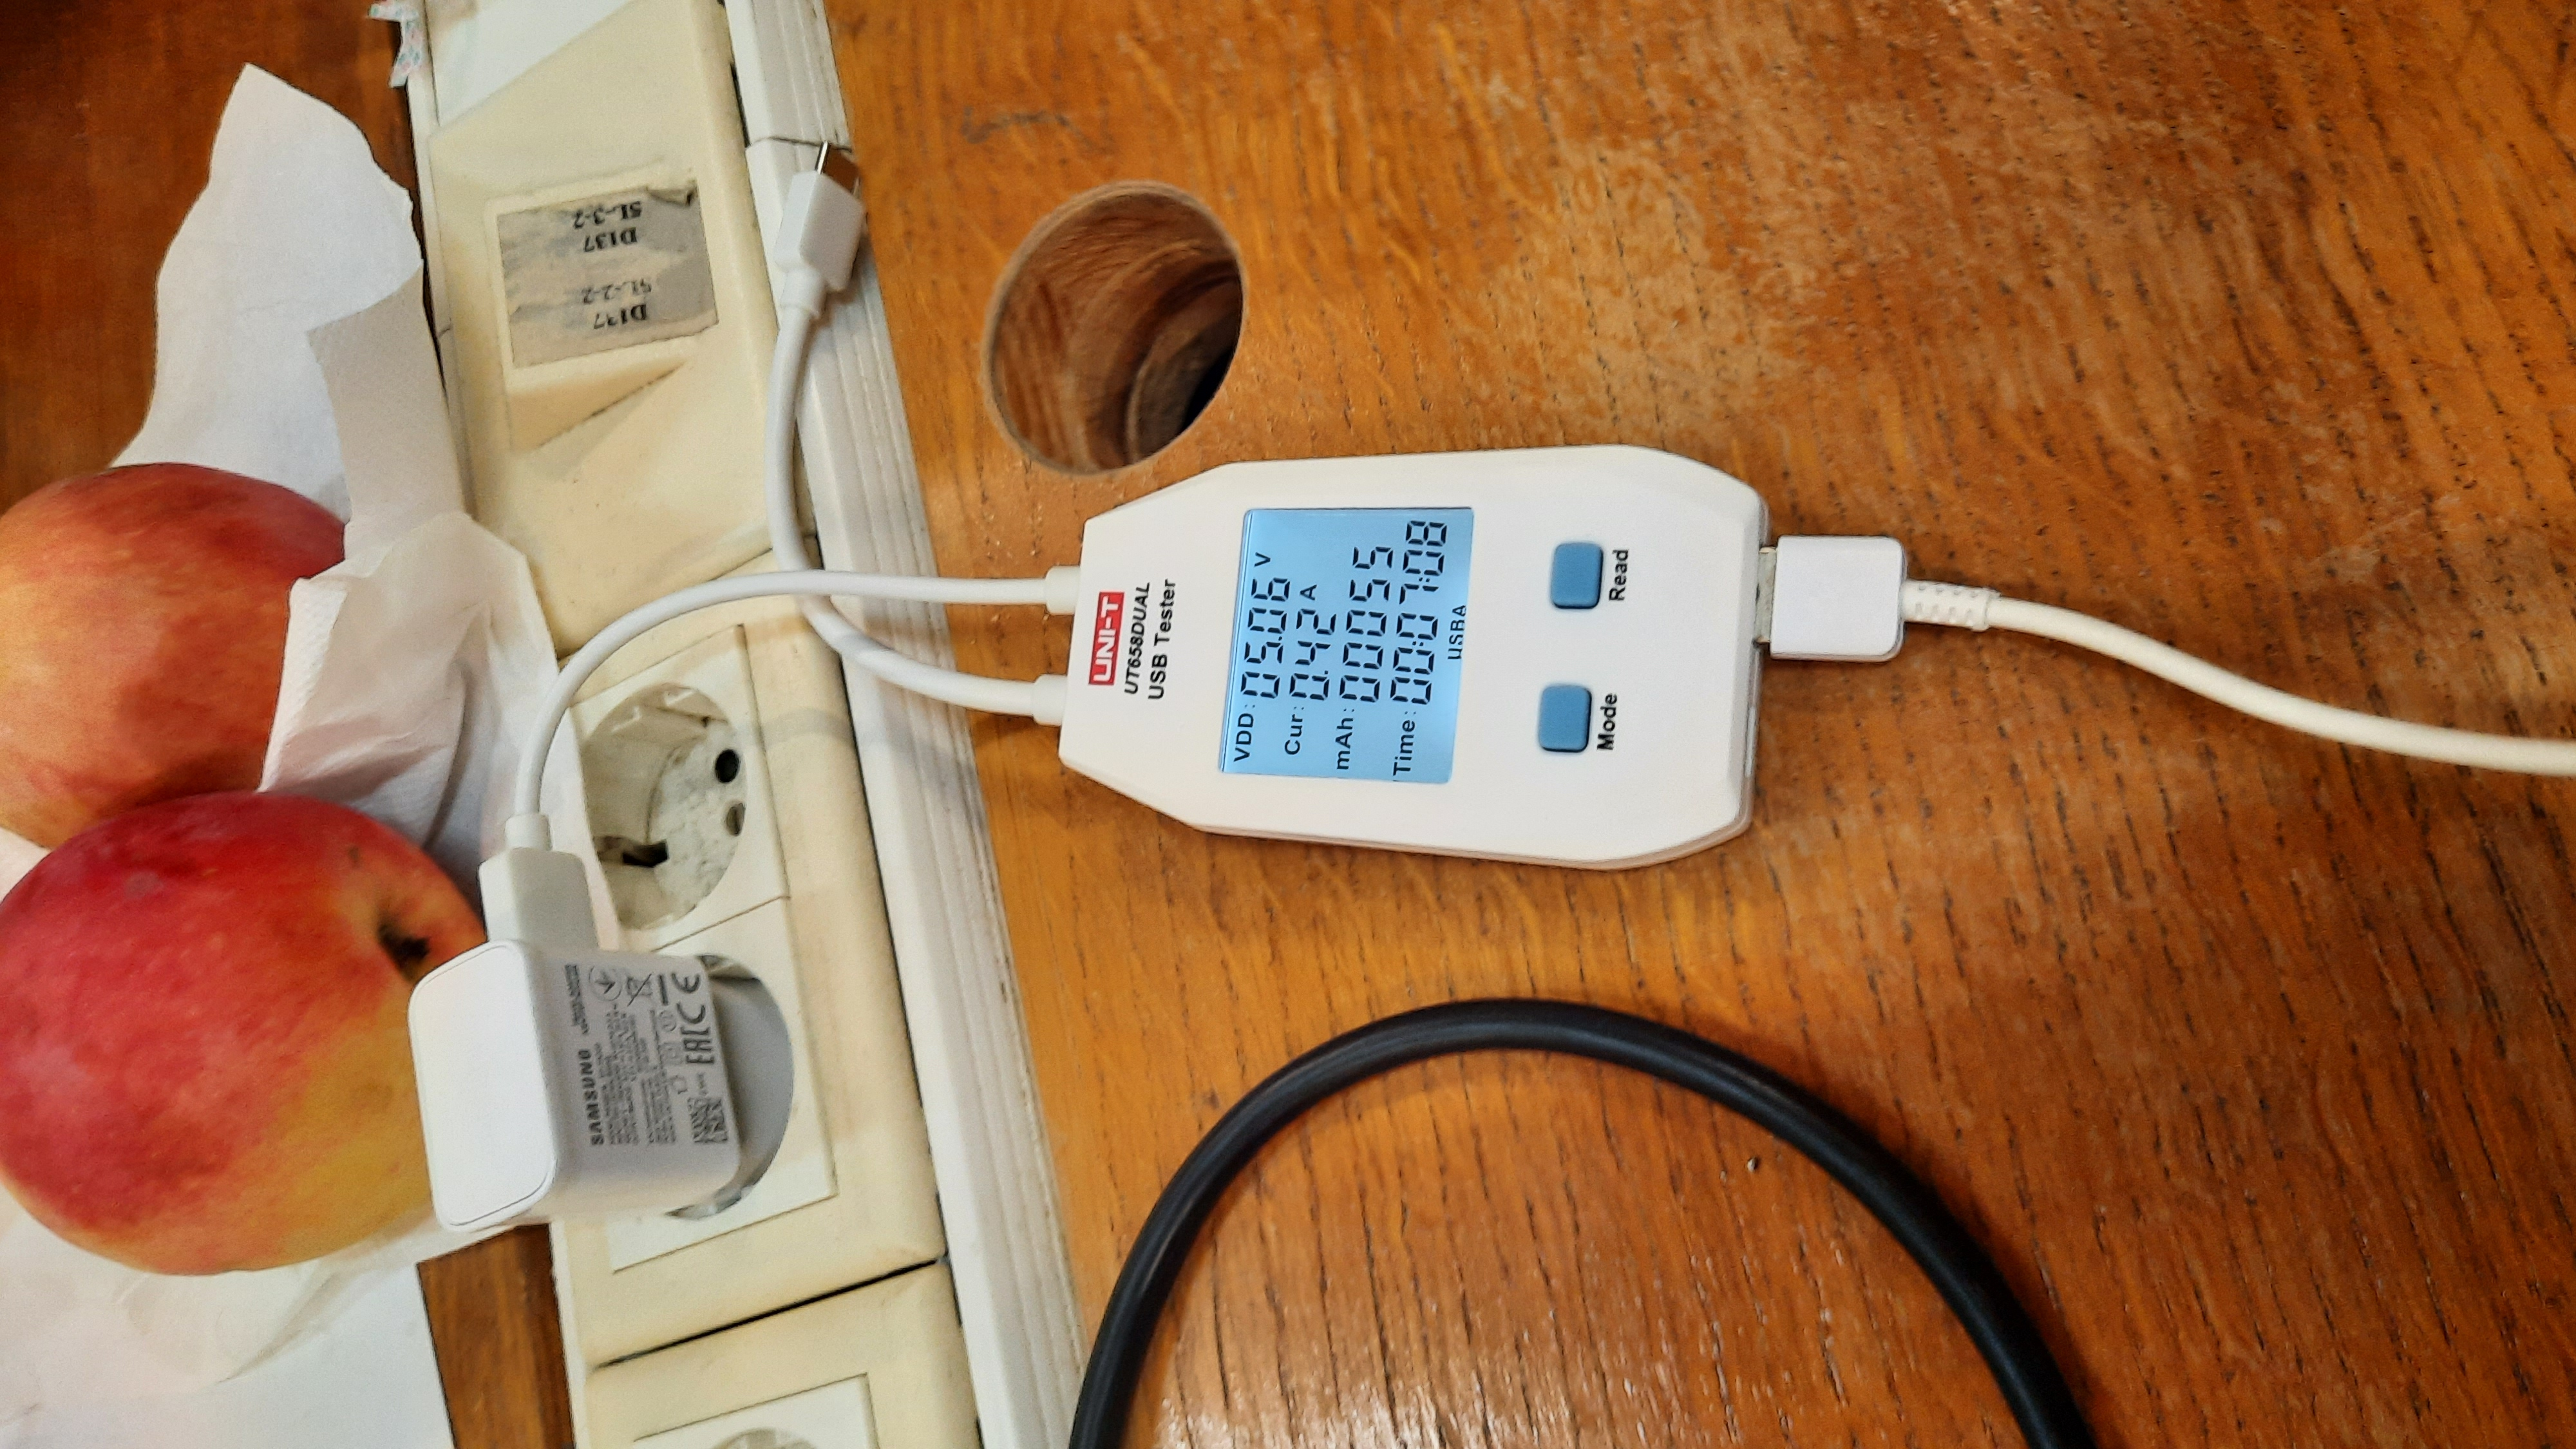
\includegraphics[width=10 cm]{Figures/BR_TEST_03.jpg}
    \caption{Brzo punjenje, punjenje konstantnim naponom}
    \label{slk:BR_TEST_03}
\end{figure}
Punjenje baterije konstantnom strujom i konstantnim naponom prikazano je na slikama \ref{slk:BR_TEST_04} i \ref{slk:BR_TEST_03}. Može se vidjeti da sustav ima napajanje i tijekom punjenja, dakle punjač također radi ispravno. Prekidački i linearni regulatori provjereni su multimetrom te na svojim izlazima imaju napon za koji su projektirani.

Tijekom ispitivanja mjernog lanca za EDR primijećeno je da je priključak za elektrode loše kvalitete jer se je periodički gubio kontakt. Radi toga je taj priključak odlemljen, a žice za EDR su izravno zalemljene na tiskanu pločicu. Dodatno je uočen problem osciliranja pojačala, što je riješeno preuzorkovanjem i usrednjavanjem više mjerenja s ADC-a. Nakon toga su dobivena stabilna mjerenja koja su odgovarala očekivanim rezultatima.

Ispravnost PPG senzora nije nažalost mogla biti verificirana jer je tijekom postupka montaže senzor bio oštećen. Radi toga je na sustav spojen modul sa senzorom MAX30100, koji se od MAX30101 razlikuje u tom što nema zelenu svjetleću diodu. Prikaz načina spoja modula na pločicu prikazan je na slici \ref{slk:BR_TEST_05}. Na ovaj način ispitana je razvijena programska podrška za PPG mjerenje. S obzirom da se radi o modulu, sklopovsko rješenje je očito ispravno.
\begin{figure}
    \centering
    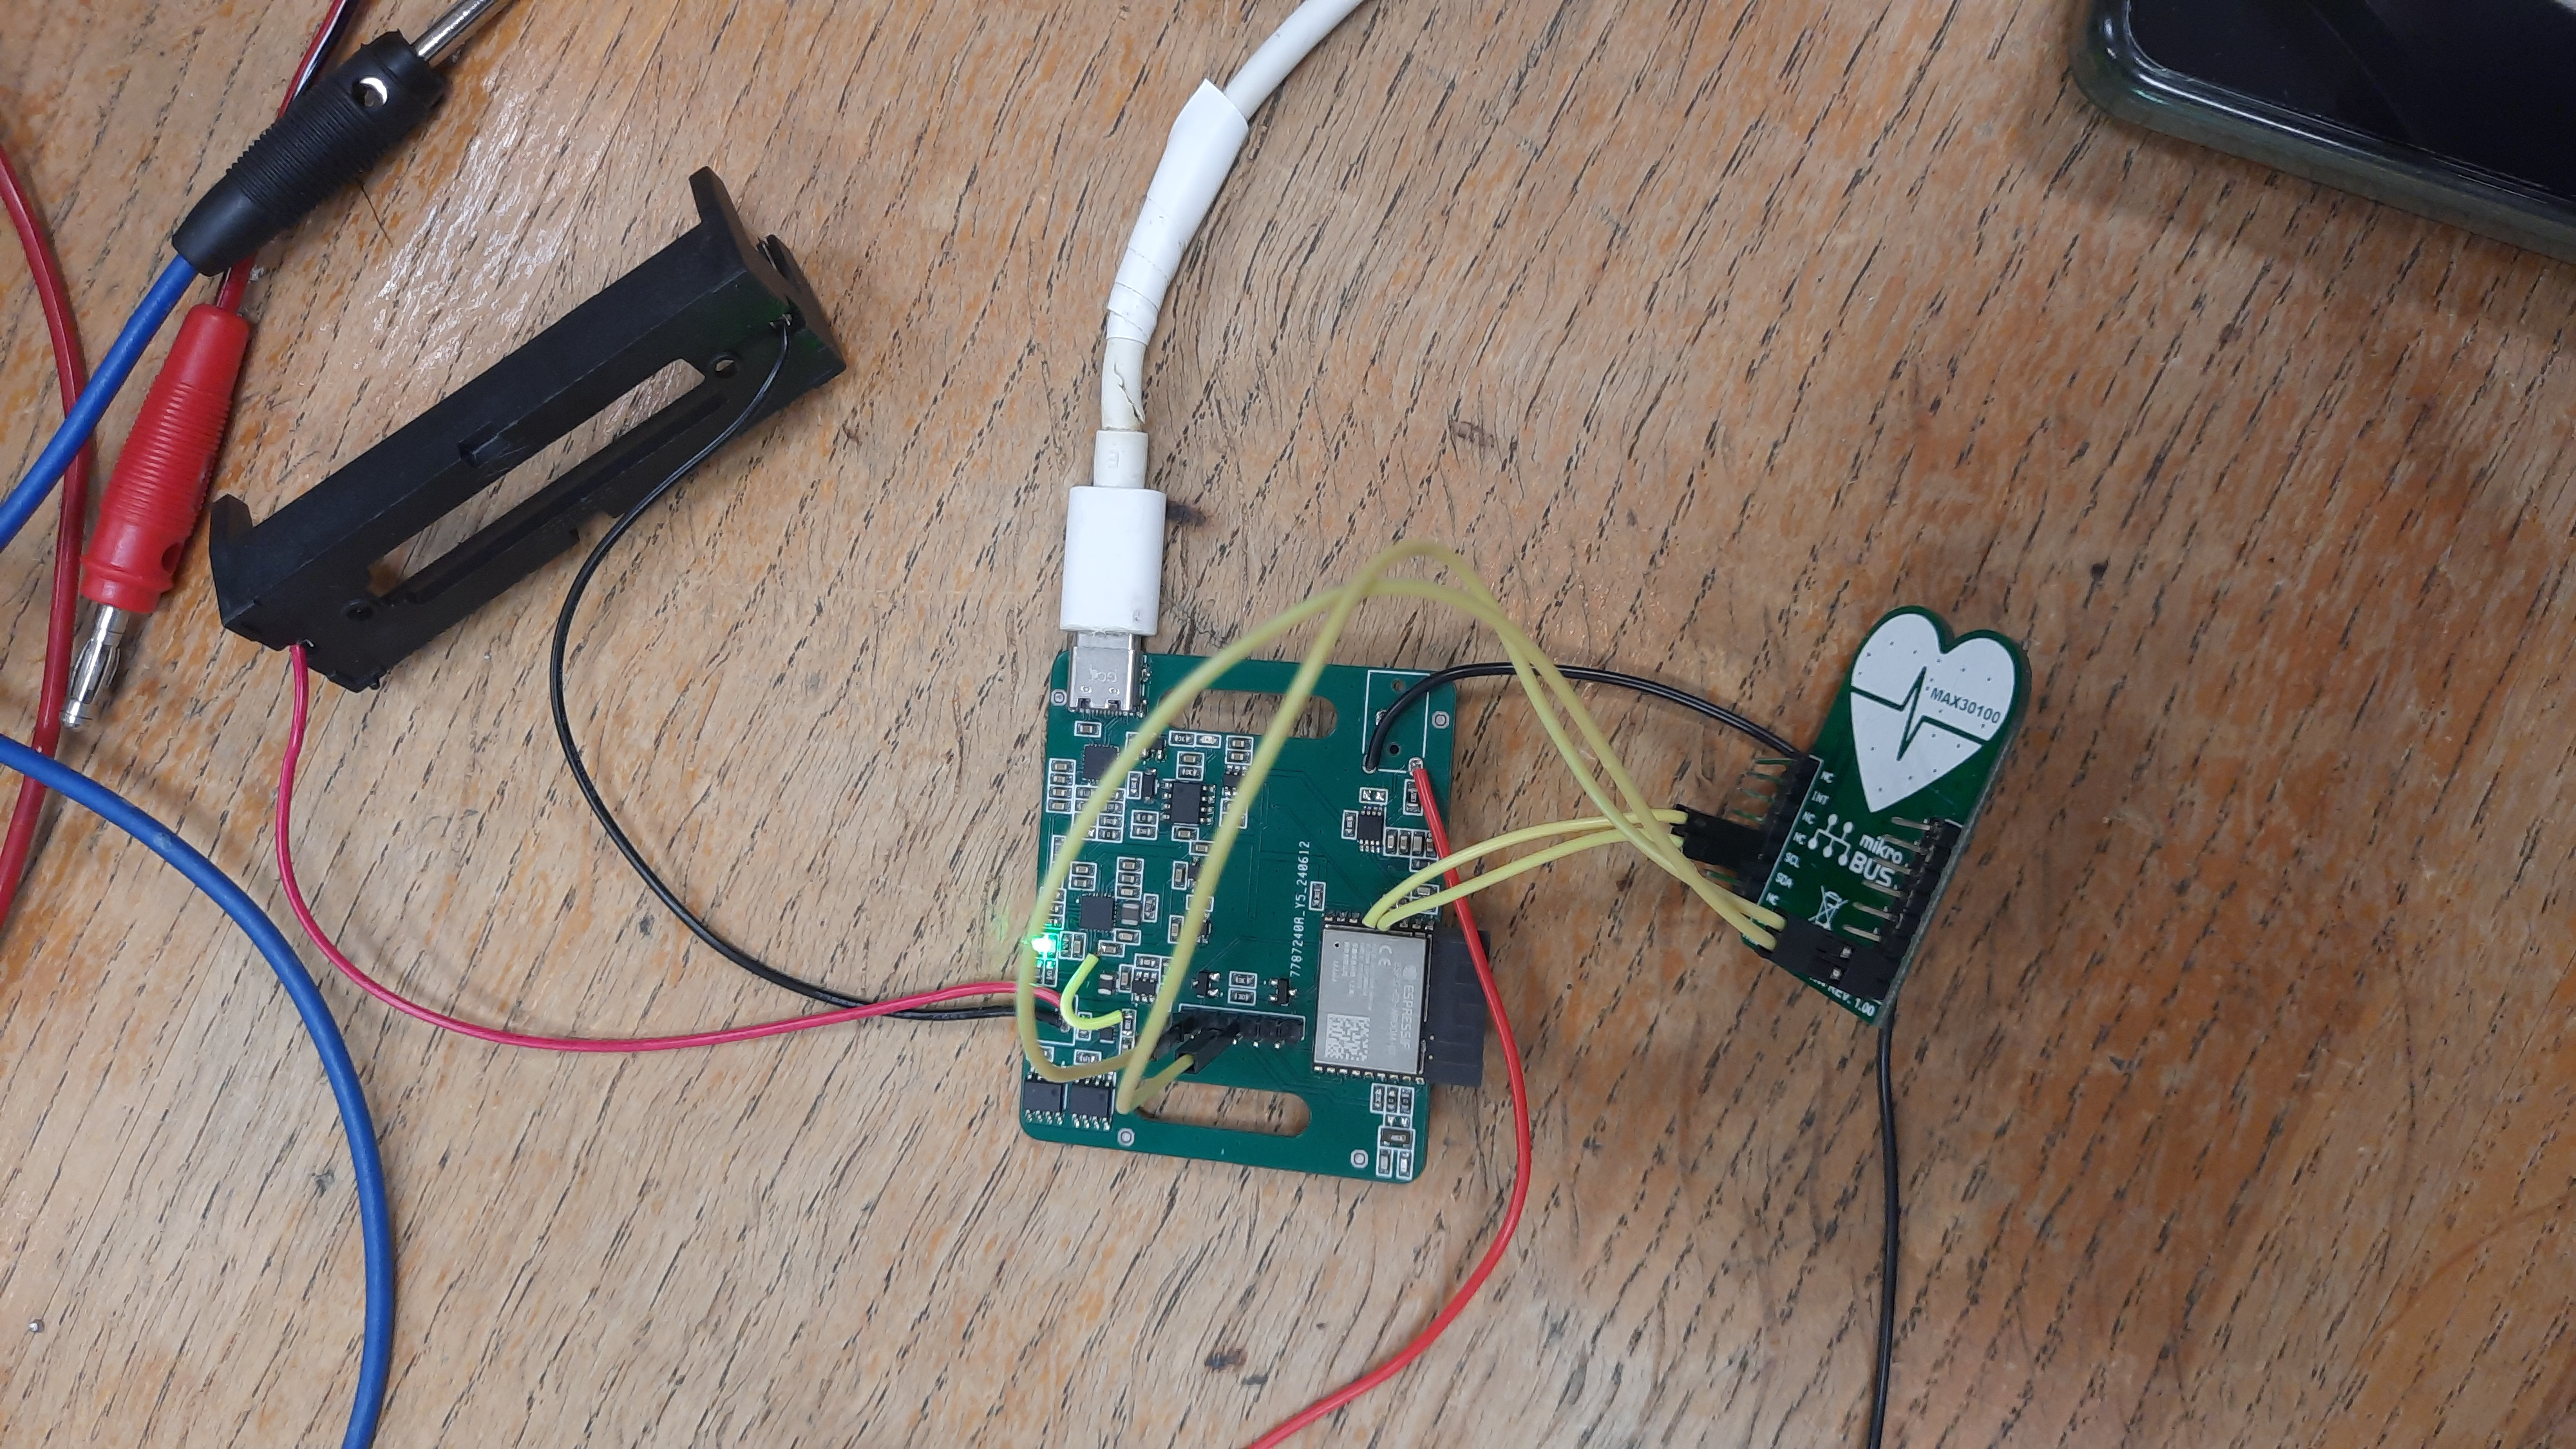
\includegraphics[width=10 cm]{Figures/BR_TEST_05.jpg}
    \caption{Spoj modula sa MAX30100 na pločicu}
    \label{slk:BR_TEST_05}
\end{figure}

ESP32 modul koji se nalazi na pločici programiran je putem USB sučelja i pokazano je da se uspješno mogao programirati, čime je verificirana njegova sklopovska ispravnost.